\chapter{手机主题推荐系统概述}

	\section{引言}
		当今的时代是信息过载(Information overload)的时代\citep{info-overload}。对于一个用户来讲互联网上充斥着大量对其无用的信息,如何从这些信息里找到用户感兴趣的信息,并把这些信息推送给用户是推荐系统面临的主要问题。推荐系统通过对用户的历史行为进行挖掘,对用户画像进行建模预测用户未来的行为。

		推荐系统的研究和很多早期的研究相关,比如认知科学(cognitive science)\citep{cognitive-science},信息检索(information retrieval)和预测理论\citep{Forecast-principle}。随着互联网的兴起,研究人员开始研究如何利用用户对物品行为数据来预测用户的兴趣并给用户做推荐\citep{cf-sn}。推荐系统开始成为一个比较独立的研究问题。到2006年为止推荐系统的研究主要集中在基于邻域的协同过滤算法,目前工业界应用最广泛、最知名的算法应该就是亚马逊开发并使用的协同过滤算法\citep{Amazon-cf}。

		近年来很多研究人员意识到推荐的时效性和多样性对于用户的体验度非常重要,而长尾效应对提高商品销售量有非常大的帮助。创建用户兴趣画像则是其中比较有效的解决途径之一,因为度量用户对物品的喜好不仅取决于用户的喜好和物品的属性,也取决于用户所处的环境,或者称做上下文(Context),上下文信息有很多类型,其中时间是一种重要的上下文信息,用户在不同的时间可能喜欢不同的物品,物品在不同的时间也有不同的流行度。因此推荐系统应该是一个动态系统,随着时间的变化会给用户不同的推荐结果\citep{temporal-cf}。

		本章接下来的内容,首先论述现有手机主题推荐系统的作用和其面临的问题,接下来详细介绍推荐系统的算法模型。

		\section{手机主题推荐系统基本概念}
		推荐系统通过分析用户-主题交互行为数据,对用户潜在感兴趣的主题打分并按优先度推荐,这里涉及到的推荐主题只局限于那些用户还没有接触过的主题,主题推荐首页如\autoref{pic:hl_recommend}所示。推荐系统的具体功能包括:
		\begin{itemize}
			\item 增加主题的销售量,具体反应在各种统计数据如购买量,点击转换率等的提升。
			\item 提升主题销售的多样性,多样性对应于长尾效应,多样性意味着推荐系统把正确的主题推送给了正确的用户,不论这个主题是热门的还是冷门的。
			\item 提升用户满意度,一个好的推荐系统能更好的明白每个人的兴趣点,做到推荐结果的千人千面,其含义包括:1,不同人对应的推荐结果不同;2,同一个人不同时间的推荐结果也应该有所不同。
		\end{itemize}
		于此同时,现有的手机主题推荐系统也存在如下问题:
		\begin{itemize}
			\item 对于一个刚刚注册成功的新用户,推荐系统往往对其所知甚少,有些时候推荐系统需要在用户购买、评价信息匮乏的情况下做出推荐。
			\item 每一分每一秒都可能有新的用户行为数据产生,而这些用户行为数据应该能够尽快作为输入传送给推荐系统作为推荐结果的参考,实现用户兴趣的无缝体验。
			\item 对于一些活跃用户,在其频繁的用户行为数据集中,可能隐藏着若干条针对小众主题的高质量行为,推荐系统应该能够准确识别出这些信息并适当的向用户展示更多相似类型的小众主题。
			\item 针对单个用户的推荐可能需要海量的数据去计算,相反,对于大多数主题其用户行为数据十分稀疏。在如何提升算法效率的同时能有效利用计算机存储空间,是推荐系统领域一个非常热门的课题。
		\end{itemize}

		\begin{figure}
		\centering
		  \framebox{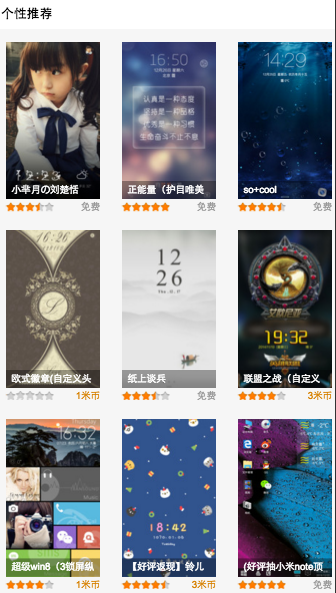
\includegraphics[scale=0.5]{figures/hl_recommend}}
		  \figcaption{主题推荐页面}
		  \label{pic:hl_recommend}
		\end{figure}

	\section{手机主题推荐系统算法模型}
		\subsection{协同过滤算法}
		协同过滤的根本原理是,人们可以从和自己有相同品味、习性的人群那里获得高质量的推荐。协同过滤算法主要研究如何聚类具有相似兴趣特征的人群并基于此做出推荐,因为算法本身是基于用户社交群体,因此往往会涉及到大规模的用户行为数据的计算。协同过滤的应用领域也很广:电子商务,金融信贷,搜素引擎,互联网企业,网络社区等需要对用户提供个性化体验的服务商。因为中国现有的人口国情,协同过滤算法往往需要面对亿万级用户和海量的用户-主题交互数据。作为输入数据,一个用户是以一个N维度的向量来表示,N代表所有的主题数量。向量内容可以为正也可为负,分别表示了用户喜欢、讨厌该主题的程度。对于热门主题,给其打分的用户会很多,其分数应该乘以一个因子u得到有效的分数,u代表所有给其打分的用户个数的倒数,大多数用户向量是稀疏的。在协同过滤算法中关键性的一步就是要选择测量的距离,描述集合相似度算法有欧氏距离、闵可夫斯基距离、汉明距离等,这里选择余弦距离公式(cosine similiarity),公式描述如下,
		其中$similarity_{uv}$代表用户u与v之间的兴趣相似度,N(u)表示用户u曾经喜欢过的物品集合,N(v)表示用户v曾经喜欢过的物品集合。

		\begin{equation}
			similarity_{uv} = \frac{|N(u)\cdot N(v)|}{||N(u)||\cdot||N(v)||}
			\label{cosine-similiarity}
		\end{equation}
		\\然后利用相似度算法把用户分类成独立的集合,每个用户有且只属于其中的一个集合,对于每个集合,取这个集合最受欢迎的top K 个主题,作为推荐内容推荐给集合的所有用户。大多数情况下协同过滤算法面都临着一个问题:最坏情况下需要遍历所有的用户和所有的主题,算法计算复杂度为O(MN),M是用户数N是主题数,解决方法可以借助一种简单的降维思想加以解决:通过去掉那些非常冷门的主题对N做降维,通过去掉那些非常不活跃的用户对M做降维,计算维度下降的代价是降低了推荐系统的准确性。

		协同过滤推荐包括User-Based CF和Item-Based CF俩种算法,User-Based CF更多的是挖掘用户之间的社交属性,而Item-Based CF更多的是挖掘物品之间的特征属性。这里根据手机主题业务的特殊性选择用Item-Based CF算法,原因包括:
		\begin{itemize}
		\item 现有手机主题共有1.1万款,线上主题约9千多款,在计算主题相似度过程中只需要维护一个1万*1万的矩阵,大约只占用了4-5GB内存,一台服务器即可承受;相反,主题用户有300万,意味着有300万*300万的矩阵,计算量太大,需要用一个spark集群完成计算,从经济效益的角度讲不可取。
		\item 手机主题一般来讲周上线不足100多款,周更新不到5\%,且可以利用增量计算方法更新item-item矩阵;相反,主题用户周增加量为10万数量级,加上用户兴趣、社交、互动的动态变化,增量计算无能为力,导致每次更新user-user矩阵的时候计算量很大。
		\item 如果用ItemCF,会只推荐与相似领域的主题的东西给用户,这样在有限的推荐列表中就可能包含了一定数量本领域不热门的item,所以ItemCF推荐长尾的能力比较强,代价是推荐多样性不足,但是对整个系统而言,因为不同的用户的主要兴趣点不同,所以系统的coverage也会很大。
		\item ItemCF的算法还可以为推荐结果做出理性的解释。如一个用户之前购买过魔兽世界的主题包,推荐系统会给其推荐魔兽争霸主题包并附上说明:因为用户曾经买过类似的主题包,并且评价分数不错。
		\end{itemize}

		\subsection{聚类模型算法}
		聚类分析(Cluster analysis)是对于统计数据分析的一门技术,和分类算法一个主要的区别就是聚类不需要人工参与打标签,基于聚类和SlopeOne预测的协同过滤方法,也可以在一定程度上解决传统协同过滤算法用户评分矩阵稀疏和冷启动问题,在降低用户评分矩阵稀疏性的同时提高目标用户最近邻居的查询速度。聚类是把相似的对象通过静态分类的方法分成不同的组别或者更多的子集(subset),这样让在同一个子集中的成员对象都有相似的一些属性,聚类结果不仅可以揭示数据间的内在联系与区别,还可以为进一步的数据分析与知识发现提供重要依据。在结构性聚类中关键性的一步就是要选择测量的距离。一个简单的测量就是使用曼哈顿距离,它相当于每个变量的绝对差值之和。该名字的由来起源于在纽约市区测量街道之间的距离就是由人步行的步数来确定的。聚类模块可以是对用户兴趣属性相似度做聚类,也可以对用户社交属性相似度做聚类,或者俩种兼有。

		在现实社会中人们的兴趣和选择往往受到身边亲朋好友的影响。在互联网中随着诸如国内的腾讯,国外的Twitter等社会网络网站的兴起,如何利用用户的社会属性做推荐是近几年推荐领域比较热门的研究问题。基于社会网络的推荐算法被称为社会化推荐(Social Recommendation)。近几年在工业界已经有了很多社会化推荐系统。最简单的社会化过滤算法是基于邻域的算法(Neighborhood-based Method)。给定用户u,令F(u)为用户u的好友集合,N(u)为用户u喜欢的物品集合。那么用户u对物品i的喜好程度定义为用户u的好友中喜欢物品i的好友个数,如公\autoref{Social-Rec}。
		\begin{equation}
			P_{vi} = \sum_{v\in F(v),i\in N(u)}^{} 1
			\label{Social-Rec}
		\end{equation}

		综合聚类模型利用了用户-用户的社会网络属性和用户-物品的兴趣属性,利用随机游走(Random Walk)\citep{Trust-walker}算法给用户做社会化推荐。Ma在提出了一个矩阵分解的算法来分解用户的社会网络矩阵和用户物品喜好矩阵,计算出用户的特征向量和物品的特征向量,并最终利用特征向量的点乘度量用户对物品的兴趣,综合模型相比较单独用社交属性和单独用兴趣属性的优点如下:
		\begin{itemize}
		\item 一般情况下用户物品矩阵的稀疏度比较高,因此仅仅利用用户-物品的兴趣属性来做协同过滤会有数据稀疏问题,造成推荐精度较差。但如果我们能通过用户的社交行为获得他的社会网络信息,就可以根据他朋友的历史行为来预测他的兴趣。
		\item 在现实社会中,人们的选择确实会受社会关系的影响,如果适当引入社会化过滤也可以增加推荐结果的用户的惊喜度和多样性。
		\end{itemize}

		聚类算法在许多领域受到广泛应用,包括机器学习,数据挖掘,模式识别,图像分析以及生物信息,手机主题推荐使用了一个叫K-均值法聚类算法,K-均值算法表示以空间中k个点为中心进行聚类,对最靠近他们的对象归类。
		\IncMargin{1em}
		\begin{algorithm}
			\SetKwData{Left}{left}\SetKwData{This}{this}\SetKwData{Up}{up}
			\SetKwFunction{Union}{Union}\SetKwFunction{FindCompress}{FindCompress}
			\SetKwInOut{Input}{input}\SetKwInOut{Output}{output}
			\Input{$k$}
			\Output{$k$个集合}
			\BlankLine
			\While{true}{
				选择聚类的个数k。\\
				任意产生k个聚类,然后确定聚类中心,或者直接生成k个中心。\\
				对每个点确定其聚类中心点。\\
				再计算其新的聚类中心。\\
				如果新旧聚类中心没有变化,跳出循环。
			}
			\Return{$k$个中心点}
		\caption{k means}\label{k-means}
		\end{algorithm}
		\DecMargin{1em}


		\subsection{SlopeOne 算法}
		SlopeOne 是一系列应用于协同过滤的算法的统称。由 Daniel Lemire和Anna Maclachlan于2005年发表的论文中提出,该算法的特点就是实现简单而高效。举例,如\autoref{tab:slopeone}所示主题2和1之间的平均评分差值为 (2+(-1))/2=0.5. 因此,主题1的评分平均比主题2高0.5。同样的,主题3和1之间的平均评分差值为3。因此,如果我们试图根据小敏对主题2的评分来预测她对主题1的评分的时候,我们可以得到 2+0.5 = 2.5。同样,如果我们想要根据她对主题3的评分来预测她对主题1的评分的话,我们得到 5+3=8。
		
		\begin{table}[htp]
		\centering
		\tabcaption{SlopeOne 示例}
		\label{tab:slopeone}
		\begin{tabular}{ |c|c|c|c| } \hline
		 顾客 & 主题1 & 主题2 & 主题3\\ \hline
		 小明 & 5 & 3 & 2 \\ \hline
		 小磊 & 3 & 4 & 未知 \\ \hline
		 小敏 & 未知 & 2 & 5 \\ \hline
		\end{tabular}
		\end{table}

		为减少过拟合的发生而实现基于SlopeOne的协同过滤算法,该方法运用更简单形式的回归表达式(f(x)=x+b) 和单一的自由参数,而不是一个主题评分和另一个主题评分间的线性回归 (f(x)=ax+b)。 该自由参数只不过就是两个主题评分间的平均差值,在某些实例当中它比线性回归的方法更有效。基于聚类算法和SlopeOne预测的协同过滤方法还可以很有效的解决数据稀疏性和推荐系统冷启动问题,实现步骤如下:
		\begin{itemize}
		\item 根据余弦相似度公式计算主题i和主题j的属性相似性,记为sims(i,j)。
		\item 根据现有主题的既得评分,组成前述的评分矩阵,计算两个主题之间的评分相似性,记为simr(i,j)。
		\item 将前两步所得结果进行线性组合,组合结果作为最终的综合相似性,记为sim(i,j):sim(i,j)=αsims(i,j)+(1-α)simr(i,j)。
		\item 对sim(i,j)按从大到小排序。取相似度最大的前$k_n$个主题作为邻居主题,从而得到目标主题的邻居主题集I={$i_1$,$i_2$,$i_3$…$k_n$},在这个邻居主题集的基础上,对目标用户运用加权SlopeOne算法进行预测,将预测评分填入空缺的评分矩阵。
		\end{itemize}

		\subsection{标签传播算法}
		Hoffman曾提出了隐语义模型(Latent Class Model)\citep{latent-cf},根据模型,我们可以认为用户并不是直接对主题产生兴趣,而是对主题所包含的几个属性特征感兴趣,而物品属于不同的类别,模型会通过用户行为学习出这些类别以及用户对类别的爱好程度,在此基础上研究人员提出矩阵分解模型,Last.fm 在线音乐平台的标签传播算法是典型的矩阵分解模型。基于内容推荐的标签传播算法通过跟踪用户所有的在线、离线、本地、远程行为,对每个用户维护一个反应其兴趣的画像,这个画像会记录用户个性化兴趣标签,让用户对自己使用的主题不断的反馈兴趣标签,然后实时的通过用户的反馈来更换用户的推荐列表,让用户越来越多的看到满意的主题包,功夫熊猫主题包的标签一共分成这么几类:心情(Mood),迎合的潜在用户人群(Audience),用户评价(Praise),铃声风格(Style), 人物态度(Attitude),背景画面(Background Picture),这些属性包括了主题方方面面的信息,可以准确描述一款主题包。推荐系统的标签一般由专职员工标注+用户标注+算法标注完成。用户标注相对于专职员工标注的特点是标签更加多样更能反映用户的长尾兴趣,但缺点是质量不高,有时候会有很多错误的标注。因此在用户标签系统中,一种方式是给用户提供一些适合于这个物品的标签供用户选择。这样做的目的有两个,首先是用户不用打字只通过点击候选标签就能完成标注的过程,其次可以提高用户标注的质量。当用户给了物品标签后就可以将标签作为物品的关键词,利用内容过滤的算法给用户做推荐。

		标签传播算法著名的应用有国外的Pandora,Lastfm和国内的虾米音乐。标签传播算法的运行步骤:
		\begin{itemize}
		\item 输入数据为半标签化的用户社交图,每个节点代表一个用户,上面标注了该用户接触过的所有主题包标签,每一个标签都对应着一个权重,一般来讲,一些用户行为包括购买、点赞对应的权重高一些,点击、浏览对应的权重低一些,其他行为的权重居中。
		\item 针对一个用户节点,把其所有的标签传播到与其相邻的其他用户节点,累加并正则化所有标签的权重。
		\item 多次迭代直到社交图上的标签达到收敛状态,输出用户社交图。
		\end{itemize}

		\subsection{最近点击模型}
		点击模型(Click Model)是对用户点击行为的建模。根据用户的历史点击信息,对用户的兴趣和行为进行建模,以对用户的未来点击行为进行预测。针对用户最近n天的行为有3项特征(Feature),分别是点击量、停留时长、滑屏频率.现有2个类别(Category),分别为用户是否购买。利用朴素贝叶斯分类器(假设特征彼此独立)计算出概率最大的那个分类,也就是求下面这个算式的最大值:
		\begin{equation}
			P(C|F1F2F3) = P(F1|C)P(F2|C)P(F3|C)P(C)
			\label{F-Measure}
		\end{equation}
		举例,假如已知某用户最近3天对某主题点击量为6次、停留时长为6秒,滑屏次数为8次,请问该用户是否会购买主体?这里面临的一个的问题是停留时长是连续变量,因此假设用户停留时长服从正态分布,通过训练样本预先计算出均值和方差,得到正态分布的密度函数。假设,没有购买的用户平均停留时长为5.855、方差为0.035,则没有购买的用户停留时长为6秒的概率为:
		\begin{equation}
			\frac{1}{\sqrt{2\pi \delta ^2}}exp\left ( \frac{-(6-5.855)^{2}}{2\delta ^{2}} \right ) \approx 1.5789
			\label{exponent}
		\end{equation}
		其他特征概率计算类似。计算结果显示,用户没有购买的概率比购买的概率高出将近10000倍,所以判断该用户对该主题不感兴趣。实验发现,对于拥有不同购物性格的用户,最近天数n的取值也不一样。有些用户总是在短时间内比较了少量的商品就下单,那么他的购物性格便是冲动型,n的取值要短些;有些用户总是在反复不停的比较少量同类商品最后才下单,那么他的购物性格便是理性型,n的取值要长些;有些用户总是长时间大量的浏览了很多商品最后才下单,那么他的购物性格便是犹豫型,n的取值要超长。

		\subsection{其他推荐算法和技术}
		用户的人口统计学特征包括了年龄,性别,工 作,学历,居住地,国籍,民族,等等。这些特征对预测用户的兴趣也有很重要的作用。对于手机主题市场更为明显,不同性别的人群兴趣不同,不同年龄的人群兴趣也不同。喜欢AK48等美女类型的主题大多是男性,喜欢刘德华等男明星类型的主题大多是女性;喜欢动漫主题的人群大多数是90后,喜欢汽车主题的人群大多是70、80后。基于用户人口统计特征的推荐的最大好处,是可以解决注册用户的冷启动(Cold Start)的问题,当一个用户刚刚注册还没有任何行为的时候,我们就可以根据他注册时提供的年龄性别等人口统计特征数据来预测他的兴趣。Krulwich 在文中\citep{demo-data}研究了如何利用大量的用户人口统计特征数据和用户行为数据来构建用户的兴趣模型的方法。首先 Krulwich 根据美国用户看电视、购物的行为将用户根据他们的人口统计学特征分成62个先验的聚类。首先找到他的聚类然后给他推荐这个聚类里的其他用户喜欢的物品。但是基于人口统计特征的推荐的主要缺点是它的推荐粒度太粗。如果我们只有用户的年龄和性别的数据,那么对于相同年龄和性别的人的推荐结果将是完全一样的。因此没有实现彻底的个性化。另外,很多用户在提交自己的年龄性别信息时,出于对自己隐私的考虑不会提供真实的信息。

	\section{手机主题推荐系统的动态特性}
		现实世界的一切事物都处在变化之中。用户的兴趣、物品的属性都是在不断的变化,一个系统中每天会有大量的新用户新物品加入;时间作为一种重要的上下文信息(Context),不同的时间用户也会有不同的兴趣,比如用户在白天和晚上的兴趣可能不同,周末和工作日的兴趣可能不同,不同的季节用户的兴趣也会有所不同。因此,合理的利用时间信息,对推荐的精准度和用户的满意度将会有很大的提升。而传统的推荐系统在设计时并没有主动的考虑到时间因素,推荐系统的动态效应表现在:
		\begin{itemize}
		\item 用户偏好随时间变化(User bias shifting):用户可能在某一天只对他喜欢的物品评分,某一天可能只对他不喜欢的物品评分。因此用户某一天的平均分是随时间变化的。
		\item 物品偏好随时间变化(Item bias shifting):物品的受欢迎程度也是随时间变化的。一款主题包在刚上线的时候的因为用户关注度小平均评分会很高,随着时间的推移,越来越多的用户参与到评分中,会使其慢慢接近真实的评分。
		\item 用户兴趣随时间变化(User preference shifting):用户在不同的时候可能有不同的兴趣,比如小孩都喜欢动漫主题包,但当他长大了可能喜欢汽车主题包。
		\item 季节效应:用户行为会受季节效应的影响。主题推荐中主要的季节效应有暑期的效应,以及一些纪念日的效应(比如国庆纪念日前后,抗日题材的主题包会受到较多的关注)。
		\end{itemize}

		为保持推荐系统的动态特性,工业界一般用数据追加的方式进行增量计算。推荐系统利用hadoop集群可以在2个小时内完成最近24小时数据的增量计算并将结果追加到现有的计算结果中,耗费的这2个小时可以用更少的时间进行增量计算并做数据追加。

	\section{推荐系统评测}
		一个好的推荐系统应该起三赢的作用:用户-找到自己感兴趣的东西;第三方设计师-增加了销量;网站-得到好的发展,提升了推荐质量。但是什么样的推荐系统才算是好的统计系统呢?这时需要有一个测评方法,常用的推荐系统测评方法见\autoref{tab:recCheck}。一个完整的推荐系统一般存在3个参与方:用户、物品提供者和网站平台.好的推荐系统不仅仅能够准确预测用户的行为,而且能够扩展用户的视野,帮助用户发现那些他们可能会感兴趣,但却不那么容易发现的东西。同时,推荐系统还要能够帮助第三方设计师将那些被埋没在长尾中的好主题介绍给可能会对它们感兴趣的用户从不同角度出发。
		\begin{table}[htp]
		\centering
		\tabcaption{推荐系统评测方法}
		\label{tab:recCheck}
		\begin{tabular}{|l|l|p{5cm}|} \hline
		 方式 & 优点 & 缺点 \\ \hline
		 离线实验 & 只需要数据集,可测试大量算法。 & 无法计算商业上关心的指标,如点击率、转化率等。 \\ \hline
		 调查问卷 & 可获得感性指标,实验风险小。 & 成本高,参与用户少,统计意义不显著,双盲实验设计困难。 \\ \hline
		 A/Btest & 可获得点击率,转化率等运营指标。& 准备周期长,设计复杂。 \\ \hline
		\end{tabular}
		\end{table}


		评测指标包括统计性指标:准确率(Precision)、召回率(Recall)、F值(F-Measure)等,也包括用户感性指标:准确度、覆盖度、新颖度、惊喜度、信任度、透明度等.一般来说评测维度分为如下几种用户维度,如果能够在推荐系统评测报告中包含不同维度下的系统评测指标,就能帮我们全面地了解推荐系统性能,找到一个看上去比较弱的算法的优势,发现一个看上去比较强的算法的缺点。

		\subsection{统计性指标}
			统计性指标包括准确率、召回率和F值,用来评价结果的质量。其中精度是检索出相关文档数与检索出的文档总数的比率,衡量的是检索系统的查准率;召回率是指检索出的相关文档数和文档库中所有的相关文档数的比率,衡量的是检索系统的查全率。正确率、召回率和 F 值是在鱼龙混杂的环境中,选出目标的重要评价指标,其定义为:
			正确率 = 提取出的正确信息条数 /  提取出的信息条数,两者取值在0和1之间,数值越接近1,正确率就越高。
			召回率 = 提取出的正确信息条数 /  样本中的信息条数,两者取值在0和1之间,数值越接近1,召回率就越高。
			F值综合了正确率和召回率的结果,见公\autoref{F-Measure}。当F值较高时则能说明试验方法比较有效。
			\begin{equation}
				F1 = \frac{2*Precision*Recall}{Precision+Recall}
				\label{F-Measure}
			\end{equation}

		\subsection{用户感性指标}
			推荐系统的新颖性。新颖的推荐是指给用户推荐那些他们以前没有听说过的物品。在一个网站中实现新颖性的最简单办法是,把那些用户之前在网站中对其有过行为的物品从推荐列表中过滤掉。评测新颖度的最简单方法是利用推荐结果的平均流行度,因为越不热门的物品越可能让用户觉得新颖。因此,如果推荐结果中物品的平均热门程度较低,那么推荐结果就可能有比较高的新颖性。

			推荐系统的惊喜度。惊喜度(serendipity)是最近这几年推荐系统领域最热门的话题,如果推荐结果和用户的历史兴趣不相似,但却让用户觉得满意,那么就可以说推荐结果的惊喜度很高,而推荐的新颖性仅仅取决于用户是否听说过这个推荐结果。

			推荐系统的信任度。信任度只能通过问卷调查的方式,询问用户是否信任推荐系统的推荐结果。提高推荐系统的信任度主要有两种方法。首先需要增加推荐系统的透明度(transparency),而增加推荐系统透明度的主要办法是提供推荐解释。只有让用户了解推荐系统的运行机制,让用户认同推荐系统的运行机制,才会提高用户对推荐系统的信任度。其次是考虑用户的社交网络信息,利用用户的好友信息给用户做推荐,并且用好友进行推荐解释。这是因为用户对他们的好友一般都比较信任,因此如果推荐的主题是好友购买过的,那么他们对推荐结果就会相对比较信任。

		\subsection{其他系统性指标}
			推荐系统的覆盖度。覆盖度描述了推荐系统对物品长尾的发掘能力,一般通过所有推荐物品占总物品的比例和所有物品被推荐的概率分布来计算,比例越大、概率分布越均匀则覆盖率越大。

			推荐系统的多样性。多样性能显著影响用户的体验。用户的兴趣是广泛的,用户可能既喜欢看《猫和老鼠》动漫的主题包,也喜欢看成龙电影的主题包。为了满足用户广泛的兴趣,推荐列表需要能够覆盖用户不同的兴趣领域,即推荐结果需要具有多样性,多样性描述了推荐列表中物品两两之间的不相似性,因此多样性和相似性是对应的。

			推荐系统的实时性。有些主题包具有很强的时效性,比如圣诞节、情人节主题包,所以需要在物品还具有时效性时就将它们推荐给用户。推荐系统的实时性包括两个方面。首先,推荐系统需要实时地更新推荐列表来满足用户新的行为变化。实时性的第二个方面是推荐系统需要能够将新加入系统的物品推荐给用户。这主要考验了推荐系统处理物品冷启动的能力。

			推荐系统的健壮性,健壮性是指推荐系统对数据异常的可控性,首先给定一个数据集和一个算法,可以用这个算法给这个数据集中的用户生成推荐列表。然后用常用的攻击方法向数据集中注入噪声数据,然后利用算法在注入噪声后的数据集上再次给用户生成推荐列表。最后通过比较攻击前后推荐列表的相似度评测算法的健壮性。如果攻击后的推荐列表相对于攻击前没有发生大的变化,就说明算法比较健壮。

	\section{本章小结}
	本章简单概述了推荐系统的主要任务和面临着的问题。从学术研究和商业应用两个角度介绍了推荐系统常用的算法,包括协同过滤、SlopeOne等若干种不同的推荐算法,在实际应用中,例如逻辑回归、协同过滤等算法本来被寄予厚望,却效果不佳;本来不起眼的最近点击和最近关注模型,反而能实现将近100\%的转化提升,这说明针对自身业务场景搭建推荐系统模型很重要。然后介绍了推荐系统的动态特性和工业界常用的解决方案。最后讨论了推荐系统的主要评测指标,在后面的各章中将会利用这些评测指标对不同的改进模型进行评测。